\documentclass[12pt]{article}
\usepackage{caption}
\usepackage{subcaption}
\usepackage{graphicx}
\graphicspath{ {images/} }
\usepackage{geometry}
\usepackage{pdfpages}
\usepackage{array}
\usepackage{amsmath}
\usepackage{url}
\usepackage[portuguese]{babel}
\usepackage{float}
%opening
\title{Exercícios de Fixação de Conceitos 2 - EFC2 - IA048}
\author{Marcelo Eduardo Pederiva RA: 122580}
\date{}
\geometry{total={210mm,297mm},
	left=20mm,right=20mm,
	bindingoffset=10mm, top=0mm,bottom=20mm}

\begin{document}

\maketitle
\section*{Parte 1 - Classificação Binária}

\subsection*{a)}

\begin{figure}[h!]
		\centering
	\begin{subfigure}{0.49\linewidth}
		\centering
		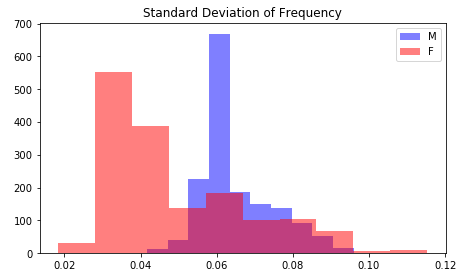
\includegraphics[width=\linewidth]{images/hist_sdf_.png}
		\caption{Standart Deviation of Frequency.}
		\label{fig:hist_sdf}
	\end{subfigure}
	\begin{subfigure}{0.49\linewidth}
		\centering
		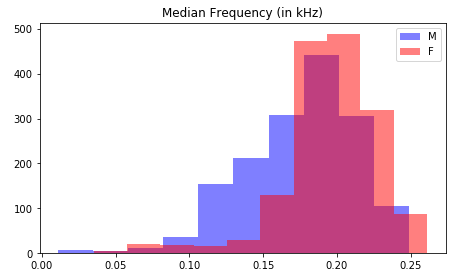
\includegraphics[width=\linewidth]{images/hist_median.png}
		\caption{Median Frequency.}
		\label{fig:hist_median}
	\end{subfigure}
	\hfill
	
	\begin{subfigure}{0.49\linewidth}
		\centering
		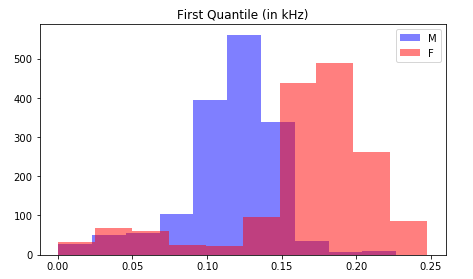
\includegraphics[width=\linewidth]{images/hist_fq.png}
		\caption{First Quantile.}
		\label{fig:hist_fq}
	\end{subfigure}
	\begin{subfigure}{0.49\linewidth}
		\centering
		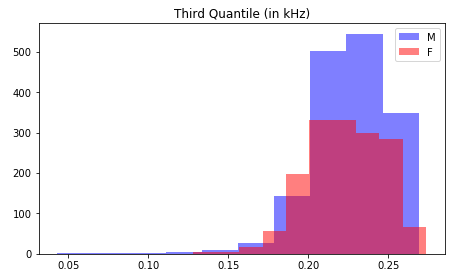
\includegraphics[width=\linewidth]{images/hist_tq.png}
		\caption{Third Quantile.}
		\label{fig:hist_tq}
	\end{subfigure}
	\hfill
	
	\begin{subfigure}{0.49\linewidth}
		\centering
		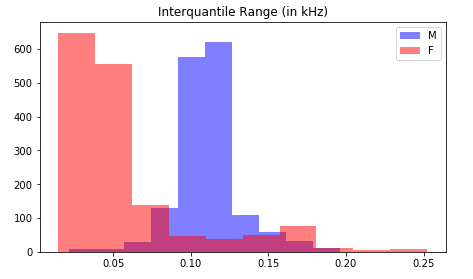
\includegraphics[width=\linewidth]{images/hist_IR.png}
		\caption{Interquantile Range.}
		\label{fig:hist_ir}
	\end{subfigure}
	\begin{subfigure}{0.49\linewidth}
		\centering
		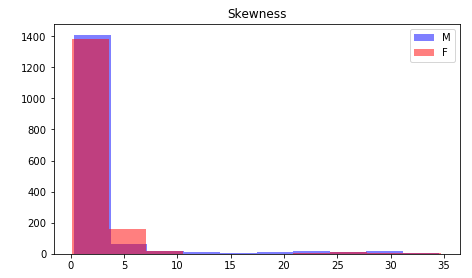
\includegraphics[width=\linewidth]{images/hist_skewness.png}
		\caption{Skewness.}
		\label{fig:hist_skewness}
	\end{subfigure}
	\caption{Histogramas}
\end{figure}

\newgeometry{left=3cm, right = 2cm, textwidth=12cm,top=1.5cm,bottom=2cm,heightrounded}

\begin{figure}[H]
	\centering
	\begin{subfigure}{0.49\linewidth}
		\centering
		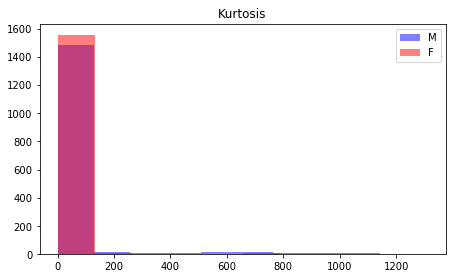
\includegraphics[width=\linewidth]{images/hist_kurtosis.png}
		\caption{Kurtosis.}
		\label{fig:hist_kurtosis}
	\end{subfigure}
	\begin{subfigure}{0.49\linewidth}
		\centering
		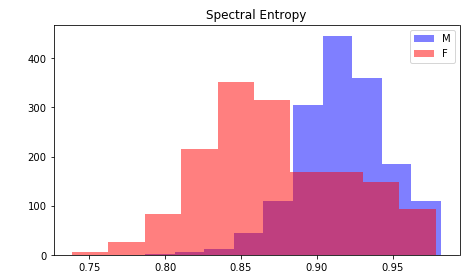
\includegraphics[width=\linewidth]{images/hist_se.png}
		\caption{Spectral Entropy.}
		\label{fig:hist_se}
	\end{subfigure}
	\hfill
	
	\begin{subfigure}{0.49\linewidth}
		\centering
		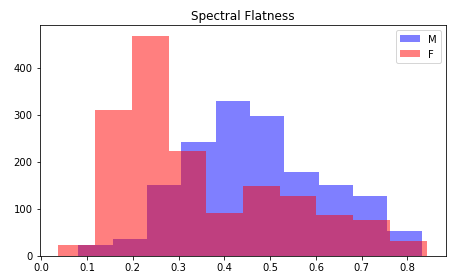
\includegraphics[width=\linewidth]{images/hist_sf.png}
		\caption{Spectral Flatness.}
		\label{fig:hist_sf}
	\end{subfigure}
	\begin{subfigure}{0.49\linewidth}
		\centering
		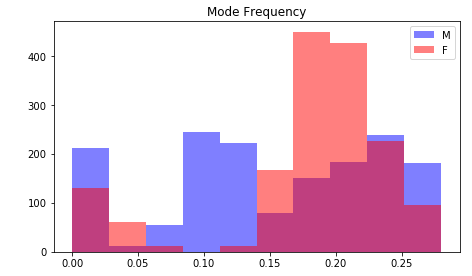
\includegraphics[width=\linewidth]{images/hist_mf.png}
		\caption{Mode Frequency.}
		\label{fig:hist_mf}
	\end{subfigure}
	\hfill
	
	\begin{subfigure}{0.49\linewidth}
		\centering
		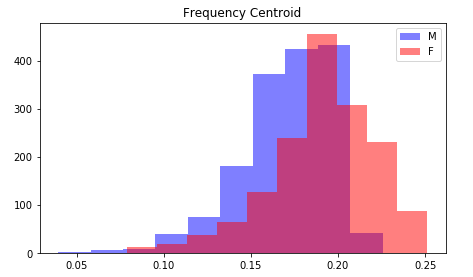
\includegraphics[width=\linewidth]{images/hist_fc.png}
		\caption{Frequency Centroid.}
		\label{fig:hist_fc}
	\end{subfigure}
	\begin{subfigure}{0.49\linewidth}
		\centering
		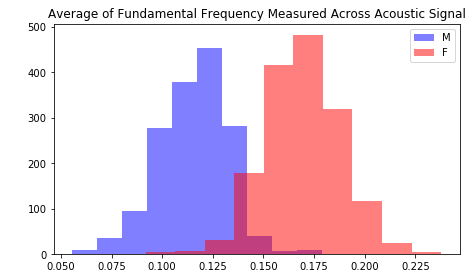
\includegraphics[width=\linewidth]{images/hist_av_ffma.png}
		\caption{Average of Fundamental Frequency Measured Across Acoustic Signal.}
		\label{fig:hist_av_ffma}
	\end{subfigure}
	\hfill
	
	\begin{subfigure}{0.49\linewidth}
		\centering
		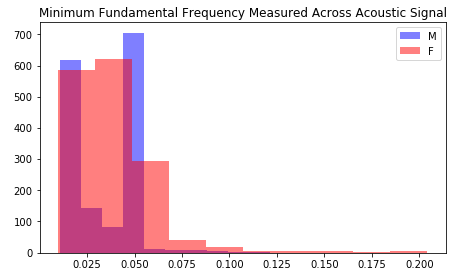
\includegraphics[width=\linewidth]{images/hist_min_ffma.png}
		\caption{Minimum of Fundamental Frequency Measured Across Acoustic Signal.}
		\label{fig:hist_min_ffma}
	\end{subfigure}
	\begin{subfigure}{0.49\linewidth}
		\centering
		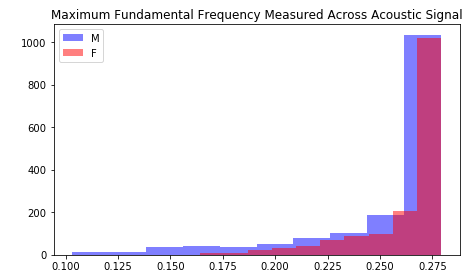
\includegraphics[width=\linewidth]{images/hist_max_ffma.png}
		\caption{Maximum of Fundamental Frequency Measured Across Acoustic Signal.}
		\label{fig:hist_max_ffma}
	\end{subfigure}
	\hfill
	\caption{Histogramas}
\end{figure}

\pagebreak
\begin{figure}[h!]
	\centering
	\begin{subfigure}{0.49\linewidth}
		\centering
		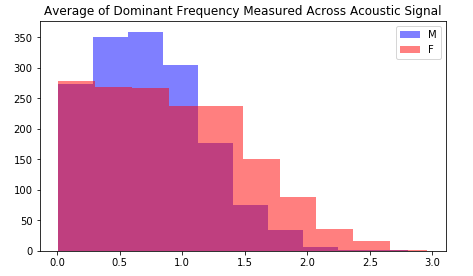
\includegraphics[width=\linewidth]{images/hist_av_dfma.png}
		\caption{Average of Dominant Frequency Measured Across Acoustic Signal.}
		\label{fig:hist_av_dfma}
	\end{subfigure}
	\begin{subfigure}{0.49\linewidth}
		\centering
		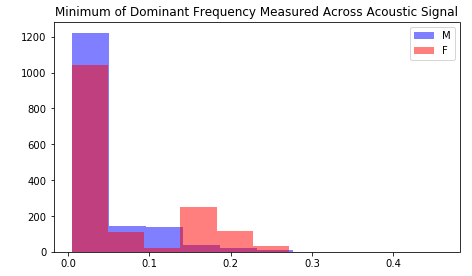
\includegraphics[width=\linewidth]{images/hist_min_dfma.png}
		\caption{Minimium of Dominant Frequency Measured Across Acoustic Signal.}
		\label{fig:hist_min_dfma}
	\end{subfigure}
	\hfill
	
	\begin{subfigure}{0.49\linewidth}
		\centering
		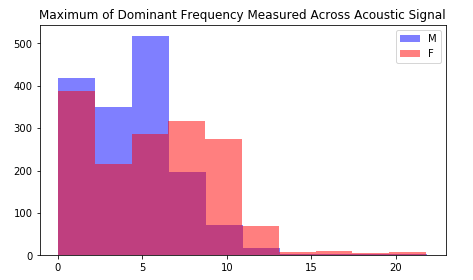
\includegraphics[width=\linewidth]{images/hist_max_dfma.png}
		\caption{Maximum of Dominant Frequency Measured Across Acoustic Signal.}
		\label{fig:hist_max_dfma}
	\end{subfigure}
	\begin{subfigure}{0.49\linewidth}
		\centering
		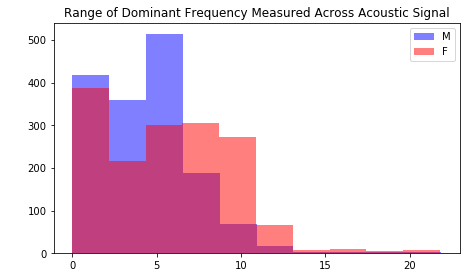
\includegraphics[width=\linewidth]{images/hist_range_dfma.png}
		\caption{Range of Fundamental Frequency Measured Across Acoustic Signal.}
		\label{fig:hist_range_dfma}
	\end{subfigure}
	\hfill
	\begin{subfigure}{0.49\linewidth}
		\centering
		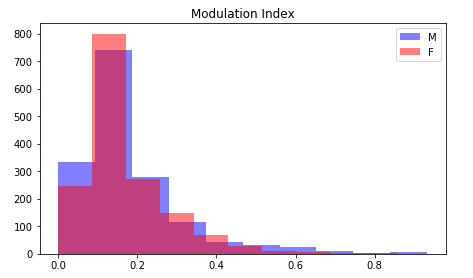
\includegraphics[width=\linewidth]{images/hist_mi.png}
		\caption{Modulation Index.}
		\label{fig:hist_mi}
	\end{subfigure}
	\caption{Histogramas}
\end{figure}

\pagebreak
Podemos observar nos histogramas acima as características de cada gênero. Na maioria dos dados, os histogramas apresentam um mesmo resultado tanto para a voz masculina como para a voz feminina. Entretanto, a análise de algumas características permitem a distinção clara do gênero da voz observado. Esta análise pode ser encontrada em algumas medidas, como: 
\begin{itemize}
	\item Desvio padrão de frequência(Fig. \ref{fig:hist_sdf})
	
	\item Primeiro quantil (Fig. \ref{fig:hist_fq})
	
	\item Intervalo Interquantil (Fig. \ref{fig:hist_ir})
	
	\item Entropia Espectral (Fig. \ref{fig:hist_se})
	
	\item Média da frequência fundamental medida através do sinal acústico (Fig. \ref{fig:hist_av_ffma}).
		
\end{itemize}

Dentre estas medidas, algumas possuem uma maior distinção entre gêneros que as outras.


\subsection*{b)}
Nessa etapa do projeto foi separado 20\% dos dados para  validação, enquanto os outros 80\% foram utilizados para treinamento do modelo de Regressão Logística.

Seguindo para a etapa de treinamento, os dados foram normalizados utilizando a técnica de normalização Min-Max.

\begin{equation}
	X' = \frac{X - \min(X)}{\max(X)-\min(X)}
\end{equation}

Com o treinamento concluído foi traçado a curva ROC (Fig. \ref{fig:roc_curve}) obtida pelo Regressor Logístico. O resultado apresentou um desempenho próximo a um classificador ideal.

\begin{figure}[h!]
	\centering
	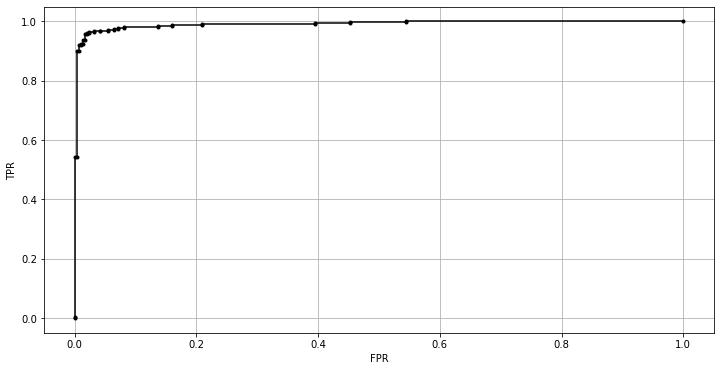
\includegraphics[width=\linewidth]{images/roc_curve.png}
	\caption{Curva ROC.}
	\label{fig:roc_curve}
\end{figure}


\pagebreak

A seguir iremos observar a influencia do \textit{threshold} de decisão em relação ao F1-Score.

\begin{figure}[h!]
	\centering
	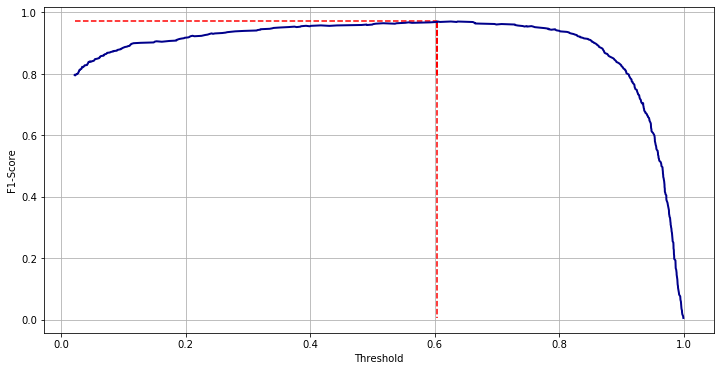
\includegraphics[width=\linewidth]{images/f1_thr.png}
	\caption{F1-Score em relação ao \textit{threshold}.}
	\label{fig:f1_thr}
\end{figure}

O gráfico acima (Fig. \ref{fig:f1_thr}) demonstra uma variação no F1-Score, conforme aumentamos o \textit{threshold} de decisão. O valor de F1-Score tende a aumentar até o limiar de \textit{threshold} = 0.6041. A partir deste ponto, conforme aumentamos o valor, o F1-Score tende a diminuir até zerar, no momento em que o \textit{threshold} de decisão iguala a 1.

\subsection*{c)}

O F1-Score define a qualidade do modelo baseado na sua precisão e a relação entre as medidas verdadeiras positivas e falso negativas (recall). Dessa forma, foi escolhido o \textit{threshold} de decisão que maximizasse o valor de F1-Score, ou seja \textit{threshold} = 0.6041. O que resultou num valor de F1-Score = 0.9707.

Com isso, frente aos dados de validação, o modelo apresentou uma acurácia de 96.53\% e a seguinte matriz de confusão (Fig. \ref{fig:conf_m}). Este resultado apresenta uma ótima precisão e uma alta certeza nas medidas.


\begin{figure}[H]
	\centering
	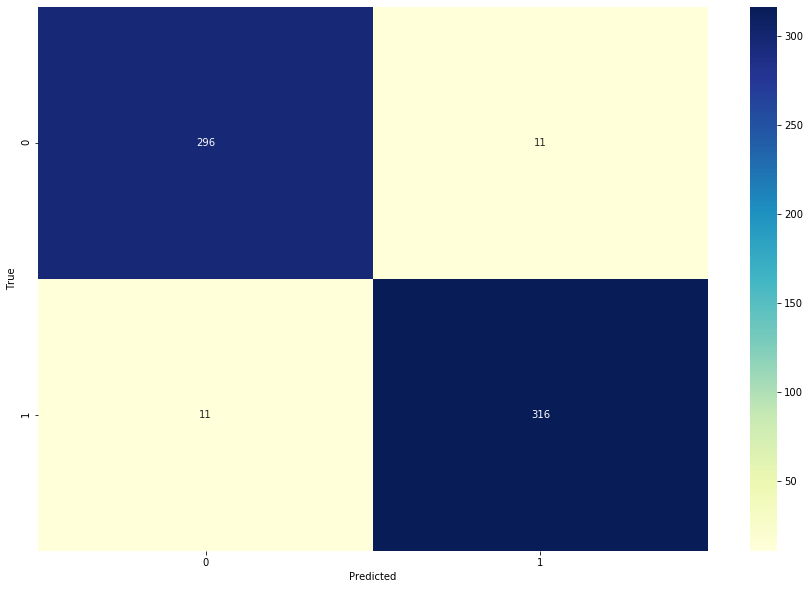
\includegraphics[width=\linewidth]{images/conf_m.png}
	\caption{Matriz de Confusão, 0 representa o gênero Feminino e 1 o Masculino.}
	\label{fig:conf_m}
\end{figure}



\section*{Parte 2 – Classificação multi-classe}

Nesta parte iremos treinar 2 modelos para caracterizar a atividade de uma pessoa através de 561 atributos. Esta atividade será diferenciada entre 6 modos:

\begin{itemize}
	\item Caminhada
	\item Subindo Escadas
	\item Descendo Escadas
	\item Sentado
	\item Em pé
	\item Deitado
\end{itemize}

\subsection*{a)}

Assim como na Parte 1, utilizaremos o modelo de Regressão Logistica para prever as atividades. Entretanto, nessa etapa será utilizado a abordagem de \textit{Softmax} para quantizar a probabilidade da classificação de cada classe, em cada uma das predições. Em outras palavras, o modelo de \textit{Softmax} irá retornar uma porcentagem de chance de cada classe ser a predita de acordo com os dados de entrada.

Com o modelo treinado, podemos observar a Matriz de Confusão gerada a partir dos dados de teste.

\begin{figure}[H]
	\centering
	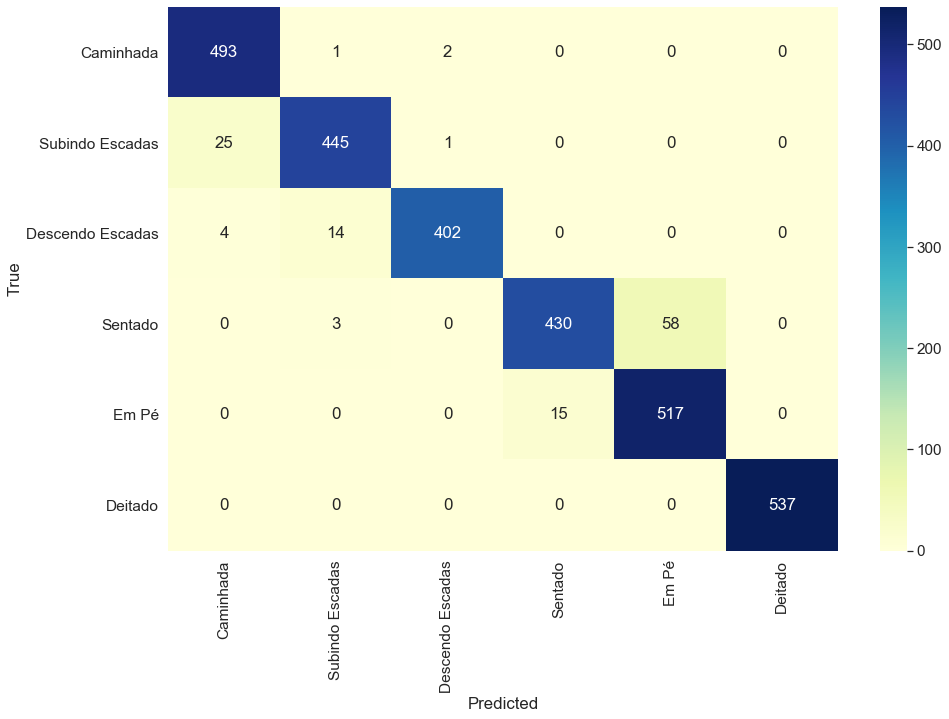
\includegraphics[width=.8\linewidth]{images/conf_m_2_lr.png}
	\caption{Matriz de Confusão da Regressão Logística.}
	\label{fig:conf_m_2_lr}
\end{figure}

A Matriz de Confusão obtida (Fig. \ref{fig:conf_m_2_lr}) demonstra que o modelo resultou em boas predições, obtendo maiores erros na predição da pessoas estarem Sentadas e Subindo escadas, no qual o modelo previu que elas estariam em Pé e Caminhando, respectivamente. 

Para a análise de desempenho do classificador de multi-classe, iremos observar os seguintes valores:

\begin{itemize}
	\item Zero-One Loss : Corresponde ao conjunto de perca de cada amostra, no qual 0 representa que todo conjunto de rotulos foi feito de forma correta e 1, totalmente incorreto.
	
	\item F1-Score Micro : Cálculo de F1-Score considerando o total de verdadeiros positivos, falso negativos e falso positivos.
	
	\item F1-Score Macro : Cálculo de F1-Score para cada classe e tirando sua média não ponderada.
	
	\item Balanced Accuracy : Acurácia balanceada, definida como a média de Recall obtido para cada Classe.
\end{itemize}

Como podemos observar abaixo, o modelo de Regressão Logistica com \textit{Softmax} apresentou uma ótima acurácia e precisão na classificação de multi-classe. 

\begin{center}
	Zero-One Loss = 0.0417
	
	F1-Score Micro = 0.9583
	
	F1-Score Macro = 0.9581
	
	Balanced Accuracy = 0.9572
\end{center}

\subsection*{b)}

Nesta etapa iremos treinar um modelo utilizando a técnica de \textit{k-nearest neighbors}(KNN) para realizar as mesmas predições.

Inicialmente iremos observar a influência do valor de k vizinhos no modelo KNN.

\begin{figure}[H]
	\centering
	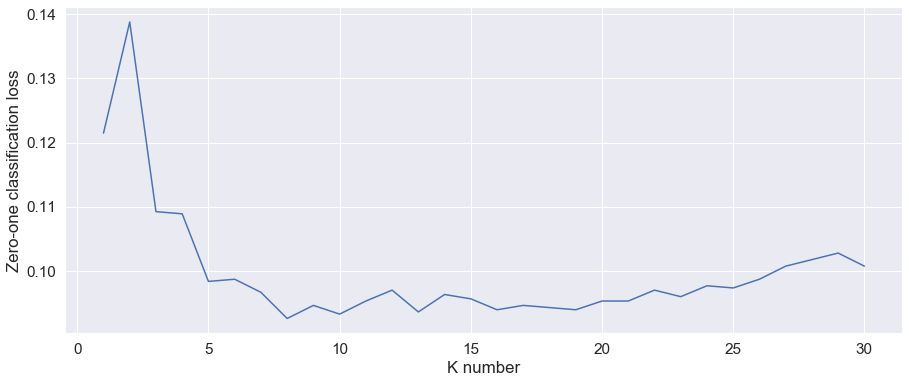
\includegraphics[width=\linewidth]{images/k_values.png}
	\caption{Resultado do treinamento com diferentes k vizinhos.}
	\label{fig:k_values}
\end{figure}

Como podemos observar na Figura \ref{fig:k_values}, o modelo possui uma variação no erro de predição conforme aumentamos o valor de k vizinhos. Esta curva tem um mínimo em k = 8 e tende a aumentar conforme aumentamos o valor de k.

Sendo assim, foi escolhido o valor de k=8 para a predição do modelo. Este valor resultou na matriz de confusão apresentada na Figura \ref{fig:conf_m_2_k}.

\begin{figure}[H]
	\centering
	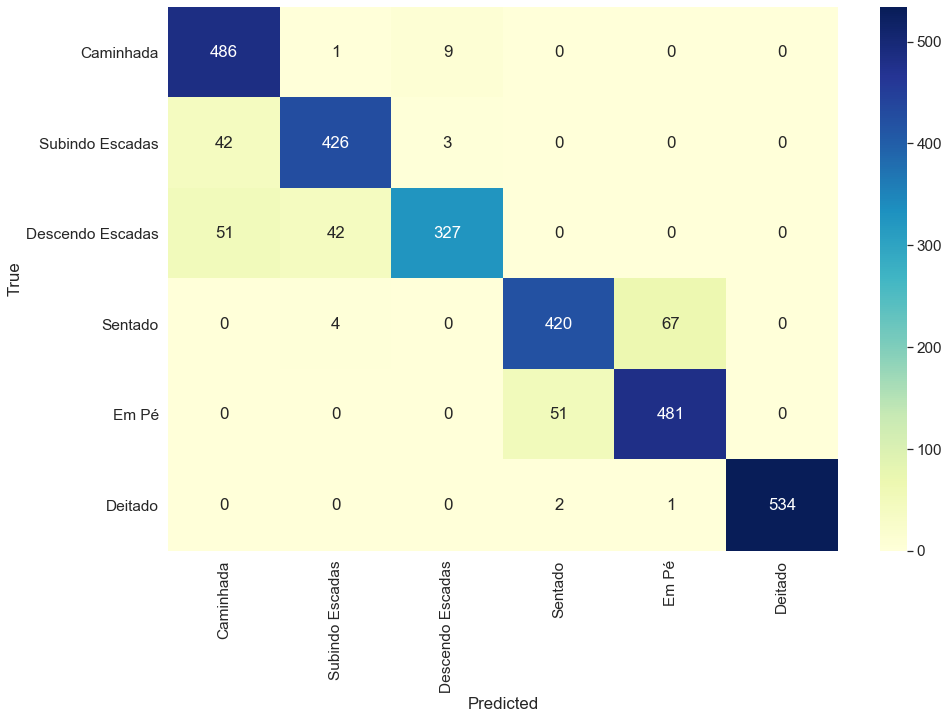
\includegraphics[width=.7\linewidth]{images/conf_m_2_k.png}
	\caption{Matriz de Confusão da técnica de KNN.}
	\label{fig:conf_m_2_k}
\end{figure}

Abaixo podemos observar o desempenho do modelo pelas as métricas de desempenho apresentadas no item a).

\begin{center}
	Zero-One Loss = 0.0926
	
	F1-Score Micro = 0.9074
	
	F1-Score Macro = 0.9045
	
	Balanced Accuracy = 0.9028
\end{center}

\subsection*{Comparação}

Matriz de confusão
\begin{figure}[H]
	\begin{subfigure}{0.49\linewidth}
		\centering
		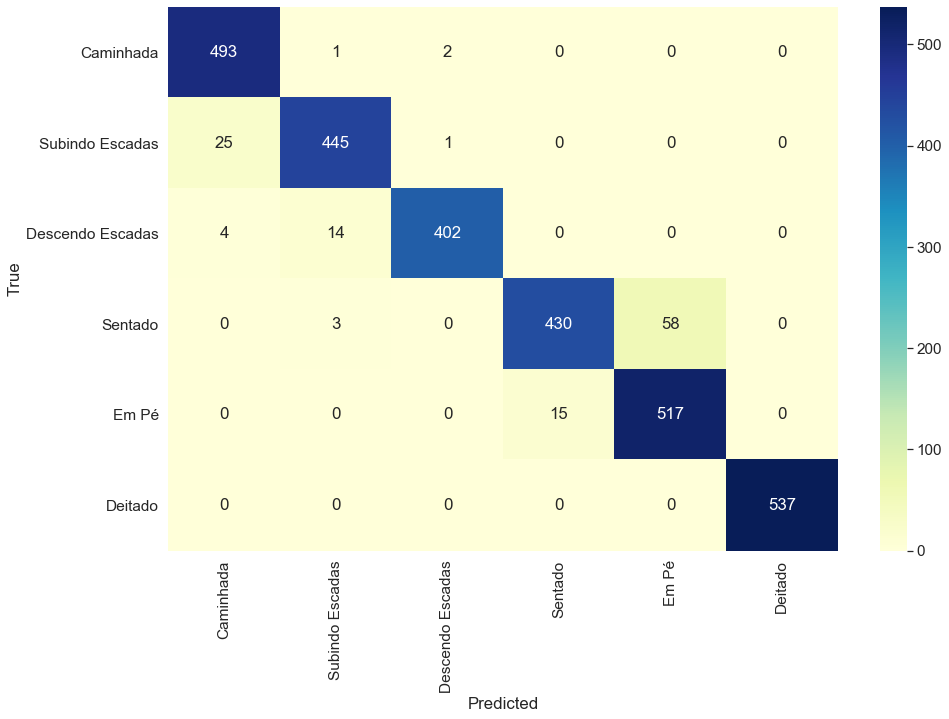
\includegraphics[width=\linewidth]{images/conf_m_2_lr.png}
		\caption{Regressão Logistica com Softmax.}
		\label{fig:conf_m_2_lr_c}
	\end{subfigure}
	\hfill
	\begin{subfigure}{0.49\linewidth}
		\centering
		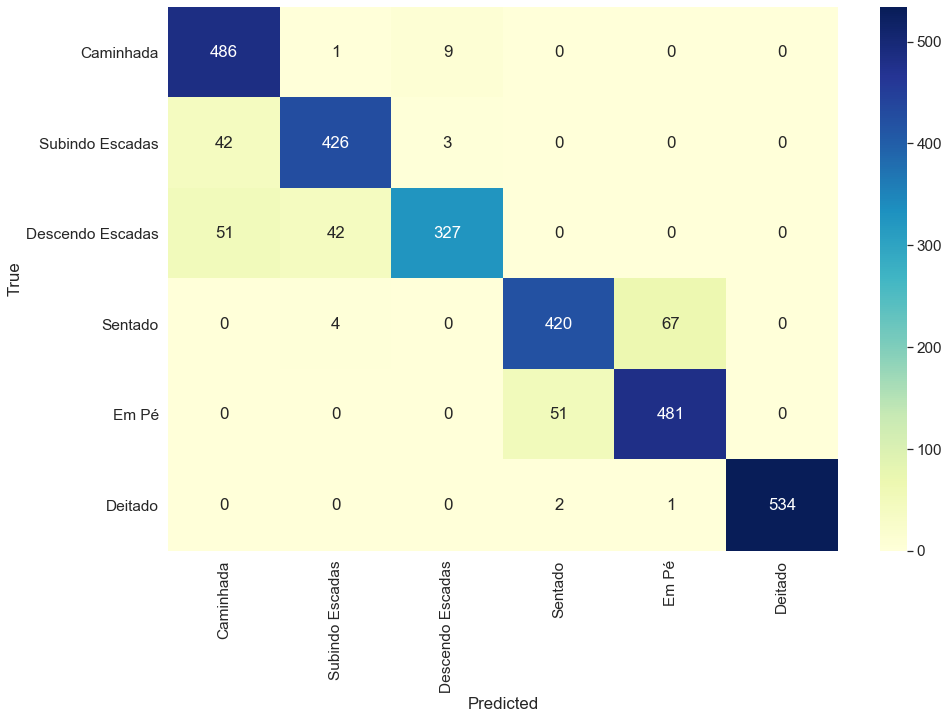
\includegraphics[width=\linewidth]{images/conf_m_2_k.png}
		\caption{KNN com k=8.}
		\label{fig:conf_m_2_k_c}
	\end{subfigure}
	\caption{Matrizes de Confusão}
	\label{fig:comp}
\end{figure}

Podemos observar na Figura \ref{fig:comp} que apesar da técnica KNN apresentar um bom resultado, a Regressão Logística ainda teve um desempenho melhor, apresentando um menor numero de classificações incorretas.

Abaixo, na Tabela \ref{tab:comp_d}, observamos que o modelo de Regressão Logística com \textit{Softmax} se sobressai no desempenho da classificação de multi-classe quando comparado com a técnica de \textit{K-Nearest Neighbors}. Porém, mesmo tendo um desempenho inferior, o KNN ainda apresentou uma ótima acurácia e confiança em suas predições.

 
\begin{table}[H]
	\caption{Comparação de desempenho}
	\label{tab:comp_d}
	\begin{tabular}{c|cccc}
		& Zero-One Loss & F1-Score Micro & F1-Score Macro & Balanced Accuracy \\ \hline
		Regressão Logística & \textbf{0.0417}        & \textbf{0.9583}         & \textbf{0.9581}         & \textbf{0.9572}            \\ \hline
		K-Nearest Neighbors & 0.0926        & 0.9074         & 0.9045         & 0.9028           
	\end{tabular}
\end{table}


\end{document}